\def\lf{\left\lfloor}
\def\rf{\right\rfloor}

\def\lc{\left\lceil}
\def\rc{\right\rceil}

Unfortunately, recurrence can only paint so much of the picture of a system's fragility. Particularly,
birth and death chains can be used to model real world scenarios, and the parameters governing these
scenarios are often subject to perturbation. As a result, an important part of the conception of
mathematical fragility being developed here is understanding how the birth and death chain reacts to
perturbations in its parameters. The most natural parameter to investigate first is the size of the step
when transitioning away from a particular state. Further, it is not true generally that all states of a
birth and death chain share the same classification, and so a more general measurement of the chain's
behavior is required. These measurements are \emph{hitting times}.
\begin{definition}
    Suppose that $X_n$ is a Markov chain with state space $\mathcal{S}$. The \emph{hitting time} from
    $i \in \mathcal{S}$ to $j \in \mathcal{S}$ is the expected amount of time required for the chain to
    achieve state $j$ given that its initial position is $i$.
\end{definition}

In order to investigate how hitting times respond to perturbations in step size, it is first helpful to
simplify the scenario, imposing that the state space be $\N$ and that each step has size $s$. Further,
let $h_s(x)$ be the hitting time to $0$ given an initial position $X_0 = x$, under the fixed step size
$s$. Returning to the metaphor of a walker, the quantity $h_s(x)$ should represent the expected amount
of time for a person initially positioned at time $x$ to reach the origin assuming a step size of $s$.
Put differently, $h_s(x)$ somehow quantifies how efficiently the chain can move from $x$ to $0$.

As such, there are a number of quantities of interest involved in the investigation of this particular
system's fragility:
\begin{itemize}
    \item   $h_s(x)$ --- the expected amount of time for the chain to hit $0$ from initial position $x$
        under a fixed step size $s$.
    \item   $\frac{\partial\, h_s(x)}{\partial\, s}$ --- the instantaneous change in hitting time to $0$
        with respect to change in the step size $s$. If this is a negative quantity, it is expected that
        increases in step size should increase the efficiency of the chain reaching $0$ from its initial
        position. In contrast, if this is a negative quantity then less efficiency is expected.
    \item   $\frac{h_s(x)}{x/s}$ --- a ratio of the hitting time to $0$ as compared to the minimum
        number of steps required to reach $0$ from initial position $x$.
    \item   $\frac{h_s(x)}{x}$ --- a ratio of the hitting time to $0$ as compared to a ``neutral''
        scenario in which the expected number of steps to reach $0$ is exactly the position $x$.
\end{itemize}

I began investigation of hitting times by first looking for a birth and death chain in which the
expected hitting time from any $n$ is given by $h_s(n) = n/s$. This is, in some sense, what is expected
to be the most minimal scenario. Doing so involved the following relationship:
\begin{equation}\label{hittingtime}
    h_s(x) = p(x)(1+h_s(x+s)) + q(x)(1+h_s(x-s)).
\end{equation}
This can be thought of as saying that the expected hitting time from $x$ is equal to the probability of
stepping in the positive direction times the associated hitting time, plus the probability of stepping
in the negative direction times its associated hitting time. However, we also know that the associated
hitting times should be one more than the hitting times from the new positions, which shows that the
associated hitting times are $1+h_s(x+s)$ and $1+h_s(x-s)$, respectively. In fact, this holds true for
all of the random walks considered here, and will be used in further investigation.

Returning now to to the scenario at hand, we can begin to deduce further information about a random walk
with such a property. By substitution into \eqref{hittingtime} using the expected hitting times, we
have that
\begin{align*}
    \frac{x}{s} &= p(x)\left(1 + \frac{x+s}{s}\right) + q(x)\left(1 + \frac{x-s}{s}\right)\\
                &= p(x) + q(x) + p(x)\, \frac{x+s}{s} + q(x) \, \frac{x-s}{s} \\
                &= 1 + p(x)\, \frac{x+s}{s} + q(x) \, \frac{x-s}{s}.
\end{align*}
Therefore,
\begin{align*}
    x &= s + p(x)(x+s) + q(x)(x-s) \\
      &= s + p(x)(x+s) + (1-p(x))(x-s) \\
      &= s + x - s + p(x)(x + s - (x - s)) \\
      &= x + 2s\, p(x).
\end{align*}
Thus, we deduce that $p(x) = 0$ should have this property. In particular, this says that $q(x) = 1$, in
which case this is the expected result. The random walk that moves in the negative direction with
probability $1$ should take the minimal amount of time to reach $0$.

This will allow us to make interesting comparisons about other random walks that we investigate. For
example, it may be interesting to find a random walk where the expected return time has no dependence on
the size of the step. A reasonable place to begin such investigation is by looking for a chain which
produces the hitting time $h_s(x) = x$. We begin again by substitution into \eqref{hittingtime}.
\begin{align*}
    x &= p(x)(1 + x + s) + q(x)(1 + x - s) \\
      &= p(x) + q(x) + p(x)(x+s) + q(x)(x-s) \\
      &= 1 + p(x)(x+s) + (1-p(x))(x-s) \\
      &= 1 + x - s + p(x)(x+s - (x - s)) \\
      &= 1 + x - s + 2s\, p(x).
\end{align*}
Thus, we deduce that $s - 1 = 2s\, p(x)$. Therefore we find that
\[
    p(x) = \frac{s-1}{2s} = \frac{1}{2} - \frac{1}{2s}.
\]
This seemed like a reasonable place to run some new simulations in order to further develop my
intuitions about hitting-times. I figured it would be beneficial to consider the hitting times of the
power-distributed birth and death chain due to my already developed familiarity with this specific
chain.

I began by updating the classes that I had written to account for a variable step size. This allowed me
to generate data sets from a variety of starting positions, storing mean hitting times as compared to
the step-size of the chain. From here, I decoupled plot generation from data analysis in order to
increase efficiency, allowing me to change \texttt{Matplotlib} parameters without regenerating data
sets. For example, the following plot represents the mean hitting time from an initial position of 100
with values of $\beta$ ranging from $-0.4$ to $0.4$ with an increment of $0.2$.

\noindent
\begin{figure}[H]
    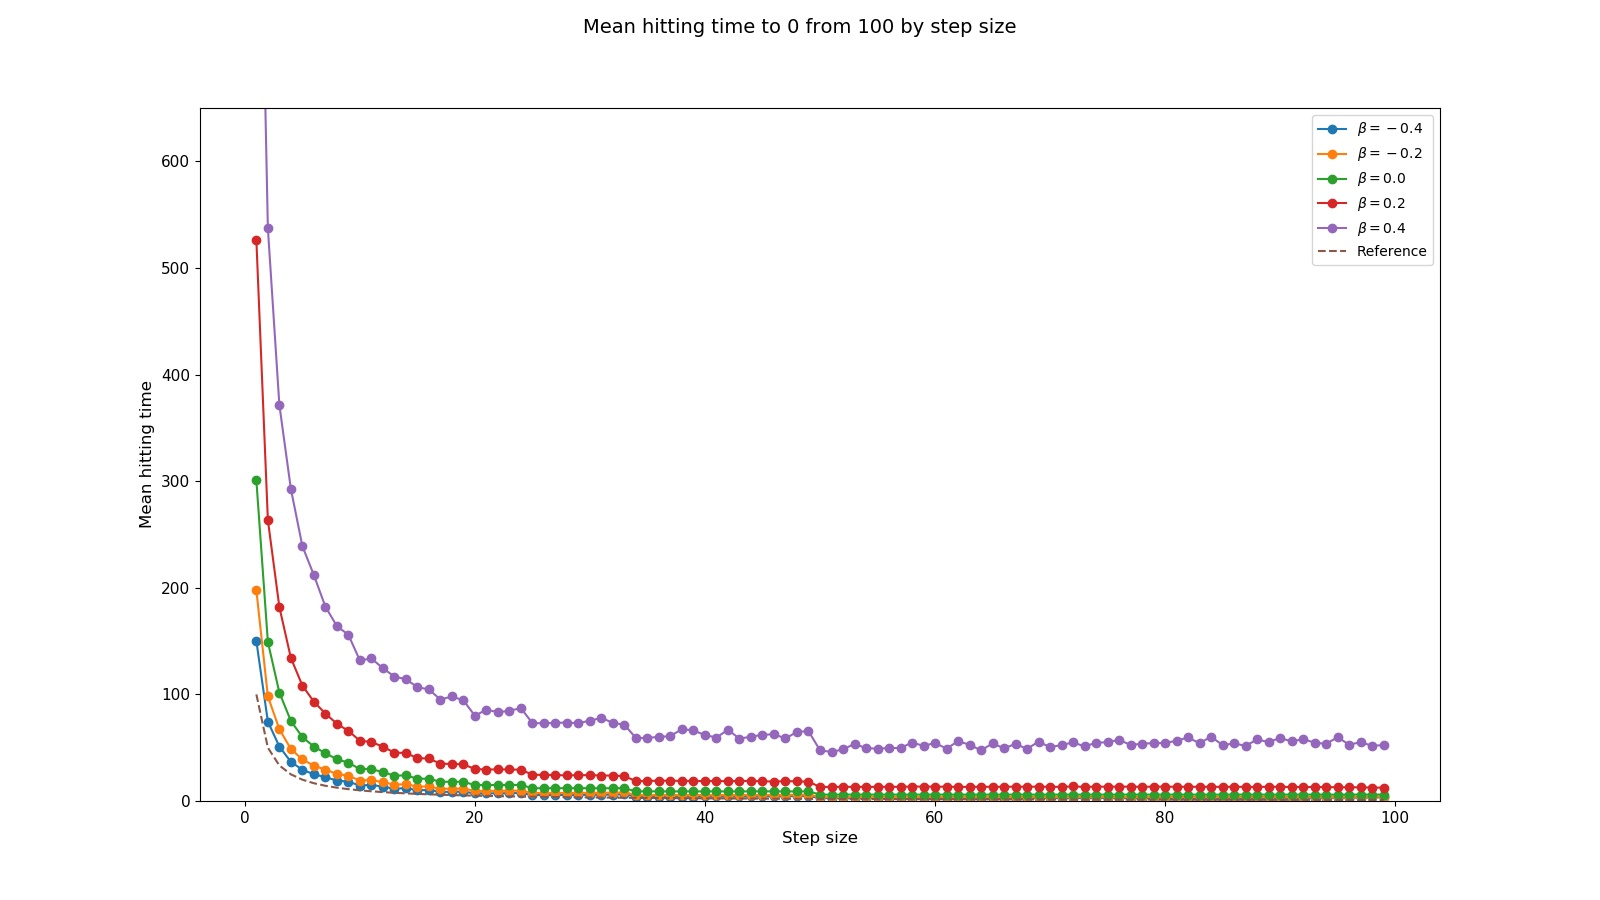
\includegraphics[width=\textwidth]{plots/hittingtimesplot1.jpg}
    \centering
\end{figure}

Further note that a reference data set is also plotted, generated by assuming that $h_s(n) = n/s$, the
``minimal'' scenario. The shape of the resultant plots suggested to me that these hitting time functions
may be scaled versions of the reference scenario, and I set out to further investigate this by
considering the ratio of hitting time functions to the minimal scenario. In other words, I set out to
plot the follwing function:
\[
    \tilde{h}_s(x) = \frac{h_s(x)}{x/s}.  
\]
Doing so in the case of an initial position of $100$ gives the following graph:

\noindent
\begin{figure}[H]
    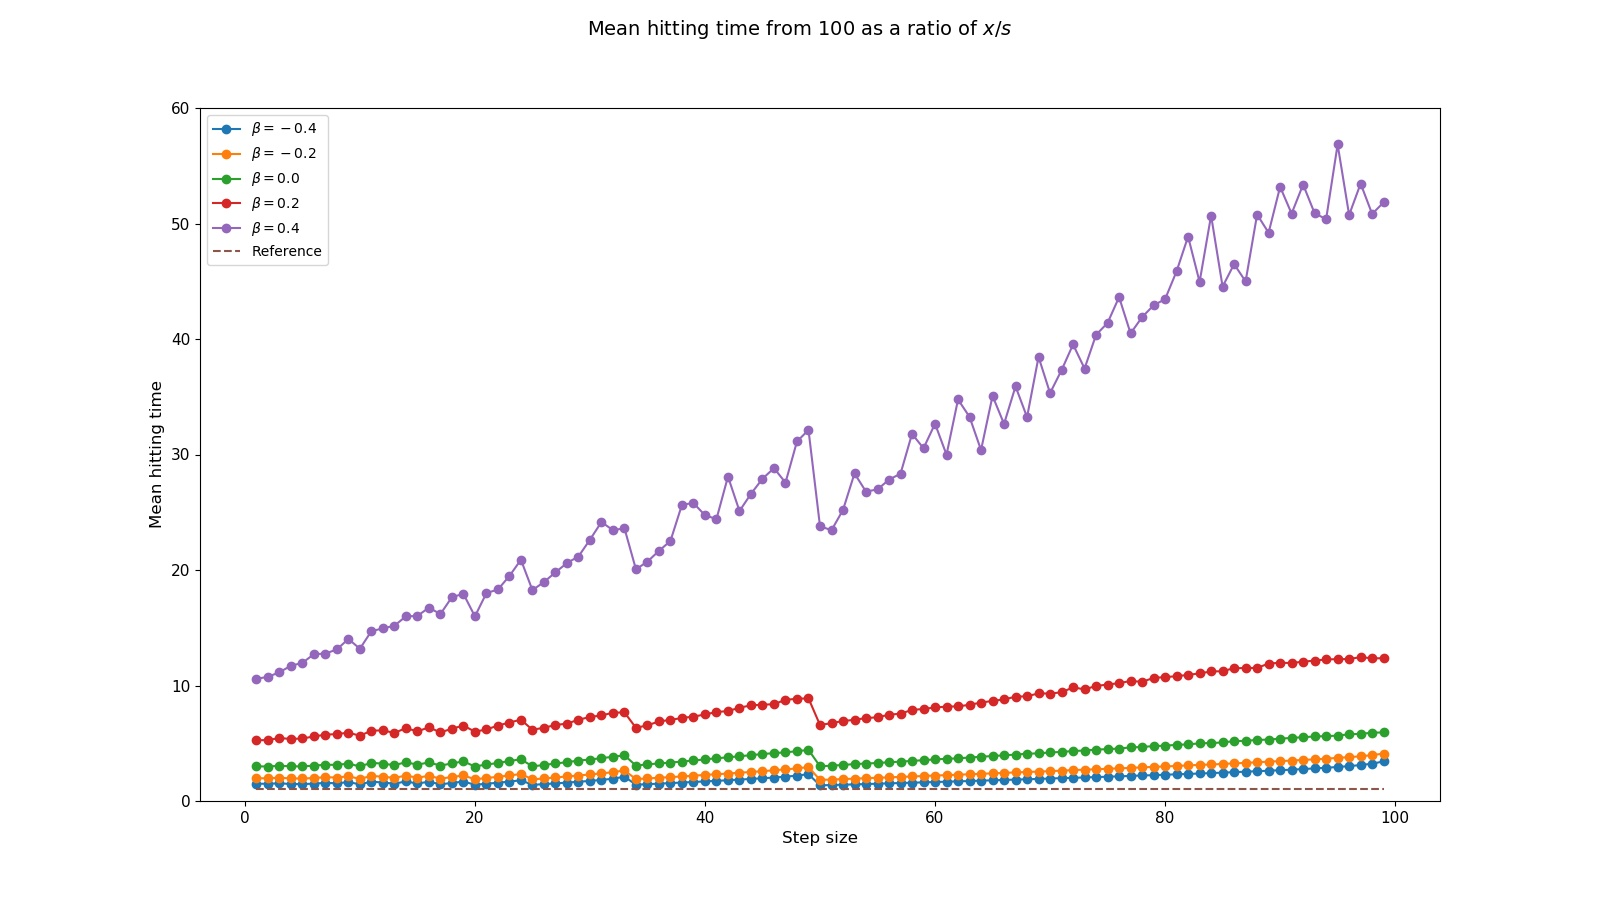
\includegraphics[width=\textwidth]{plots/hittingtimesplot2.jpg}
    \centering
\end{figure}

If the mean hitting time functions were scaled versions of the minimal reference scenario, we would
expect to see lines at constant values (representing the scaling factor). Instead, this plot reveals
that these ratios are generally increasing and so the hitting time functions are not scalings of the
reference scenario. This conclusion is further supported by similar plots generated with an initial
position of $1000$.

However, these plots illuminated an interesting subset of the step sizes where the mean hitting time
seems to instantaneously decrease. I set out to investigate the nature of this sequence, by first
estimating the step-size on the plot. By reading off approximate values, I was able to determine that
this sequence seems to be related to the division algorithm. In particular, we know by the division
algorithm that
\[
    100 = ms + r,
\]
where $s$ represents a step-size, $m$ represents some number of steps, and $r$ represents a remainder
term. Further, the division algorithm guarantees that $r < s$. We hypothesized that if it were also true
that $r < m$, then the corresponding $s$ is a member of this special subset of step-sizes. In the case
of $n=100$, those step-sizes included $50, 33, 25, 20, 16, 14, 12$, and $11$. I then cross-referenced
this sequence with the Online Encyclopedia of Integer Sequences to confirm that this sequence is given
by
\[
    s_{m} = \lf \frac{n}{m} \rf.
\]
However, further pondering led me to believe that this sequence is in fact incorrect. In particular, we
might expect there to be a drop when $s = 34$ instead of when $s = 33$, as it will require at a minimum
$3$ steps to reach $0$ when $s = 34$ as compared to a minimum of $4$ steps when $s = 33$.
Reconsideration of the division algorithm led me to the fact that if the accompanying remainder term is
non-zero, then the walk will have not quite reached the origin in $m$ steps. As a result, the
accompanying step-size is one larger. The sequence when $n=100$ thus instead contains $50, 34, 25, 20,
17, 15, 13$, and $12$. This corresponds to the sequence given by
\[
    s_m = \lc \frac{n}{m} \rc.  
\]

While this sequence of step-sizes was initially of interest due to the instantaneous-behavior, further
investigation led me to deem these sequences unhelpful. It seems that little can be learned about the
behavior of the power-distributed birth and death chain from these sequences.

The investigation of hitting times of the power-distributed chain is also hampered by the fact that when
$\beta > 1$ the mean hitting time may not always be defined. The following plot shows a variety of
different values of $\beta$ (all values less than one are plotted on the left, and all values larger
than one on the right).

\noindent
\begin{figure}[H]
    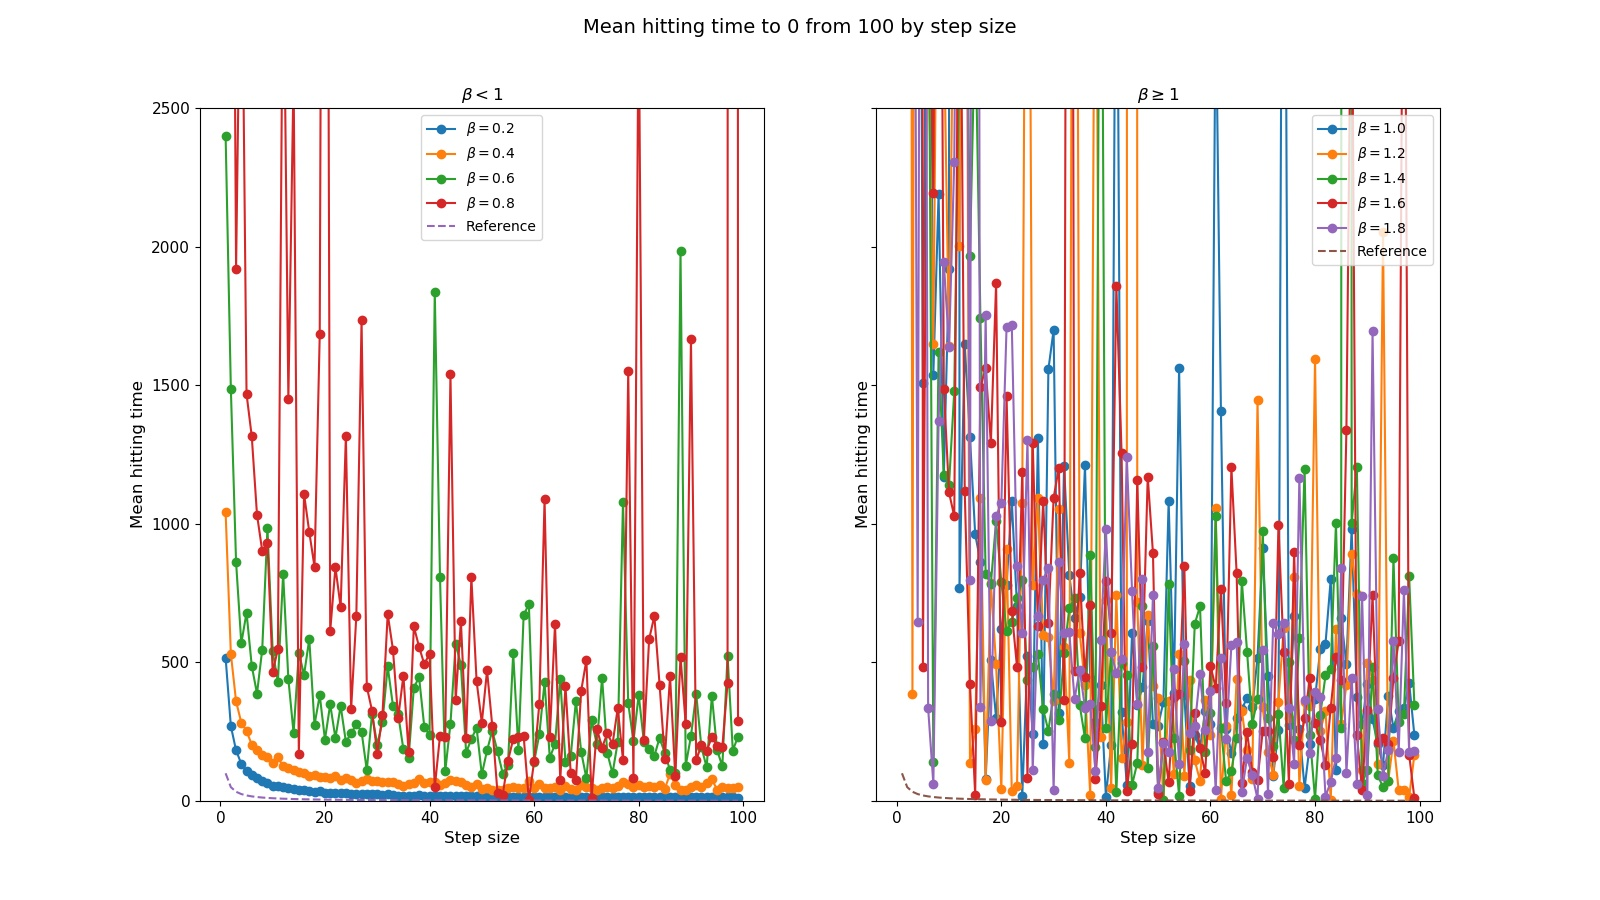
\includegraphics[width=\textwidth]{plots/hittingtimesplot3.jpg}
    \centering
\end{figure}

Notice that on the left, scattering increases greatly as $\beta$ approaches a value of $1$. Further, on
the right, there is scattering for all values of $\beta$ shown. This represents instances where the
simulation diverges away from the origin, not returning with any particular pattern. This is consistent
with the results gathered about return-times of the power-distributed chain when $\beta > 1$.

The results from the simulations on hitting times will next lead me to some analytic investigation of
hitting times. In particular, I would like to begin generalizing some of my results. For example, it may
be true that if the transition probability $p(x)$ monotonically increases to $1/2$ as $x$ approaches
infinity, then the resultant mean hitting time functions $h_s(n)$ behave similarly to the simulated
scenarios.

However, results from the simulations also show that hitting times can only capture so much information
about a given birth and death chain. In the case of the power-distributed chain, mean hitting time
cannot provide useful comparison when $\beta > 1$. As such, further investigation will need to overcome
this obstacle.
